
\chapter{Implementation}
\epigraph{The trouble with opportunity is that it always comes disguised as hard work.}%
{\textsc{---herbert v. prochnow}}


The previous chapter described the design of the Accelerate language, an
embedded DSL of operations over arrays, rich enough to express some interesting
real-world problems. This chapter details the architecture of the embedding as
well as the implementation of a backend for parallel execution on CUDA hardware.

\section{Accelerate CUDA Backend}
\subsection{Parallel Reduction}
\label{sec:parallel_reduction}

Figure~\ref{fig:tree_reduction} illustrates the basic strategy of a tree
\marginnote{tk: move to the implementation chapter}
reduction, a common and important data-parallel primitive. Within each thread
block a tree-based approach is used to reduce elements to a single value, and
multiple thread blocks each process a portion of the array in parallel. There is
no global synchronisation primitive in CUDA, because (a) it would be expensive
to build in hardware for large numbers of multiprocessors, and (b) would be
difficult for programmers to use without introducing sources of deadlock.
Instead, kernel launches serve as a global synchronisation point, so thread
blocks instead communicate their partial results by committing them to memory,
and the kernel is launched recursively until the final reduction is computed.

\begin{figure}[htbp]
    \begin{center}
        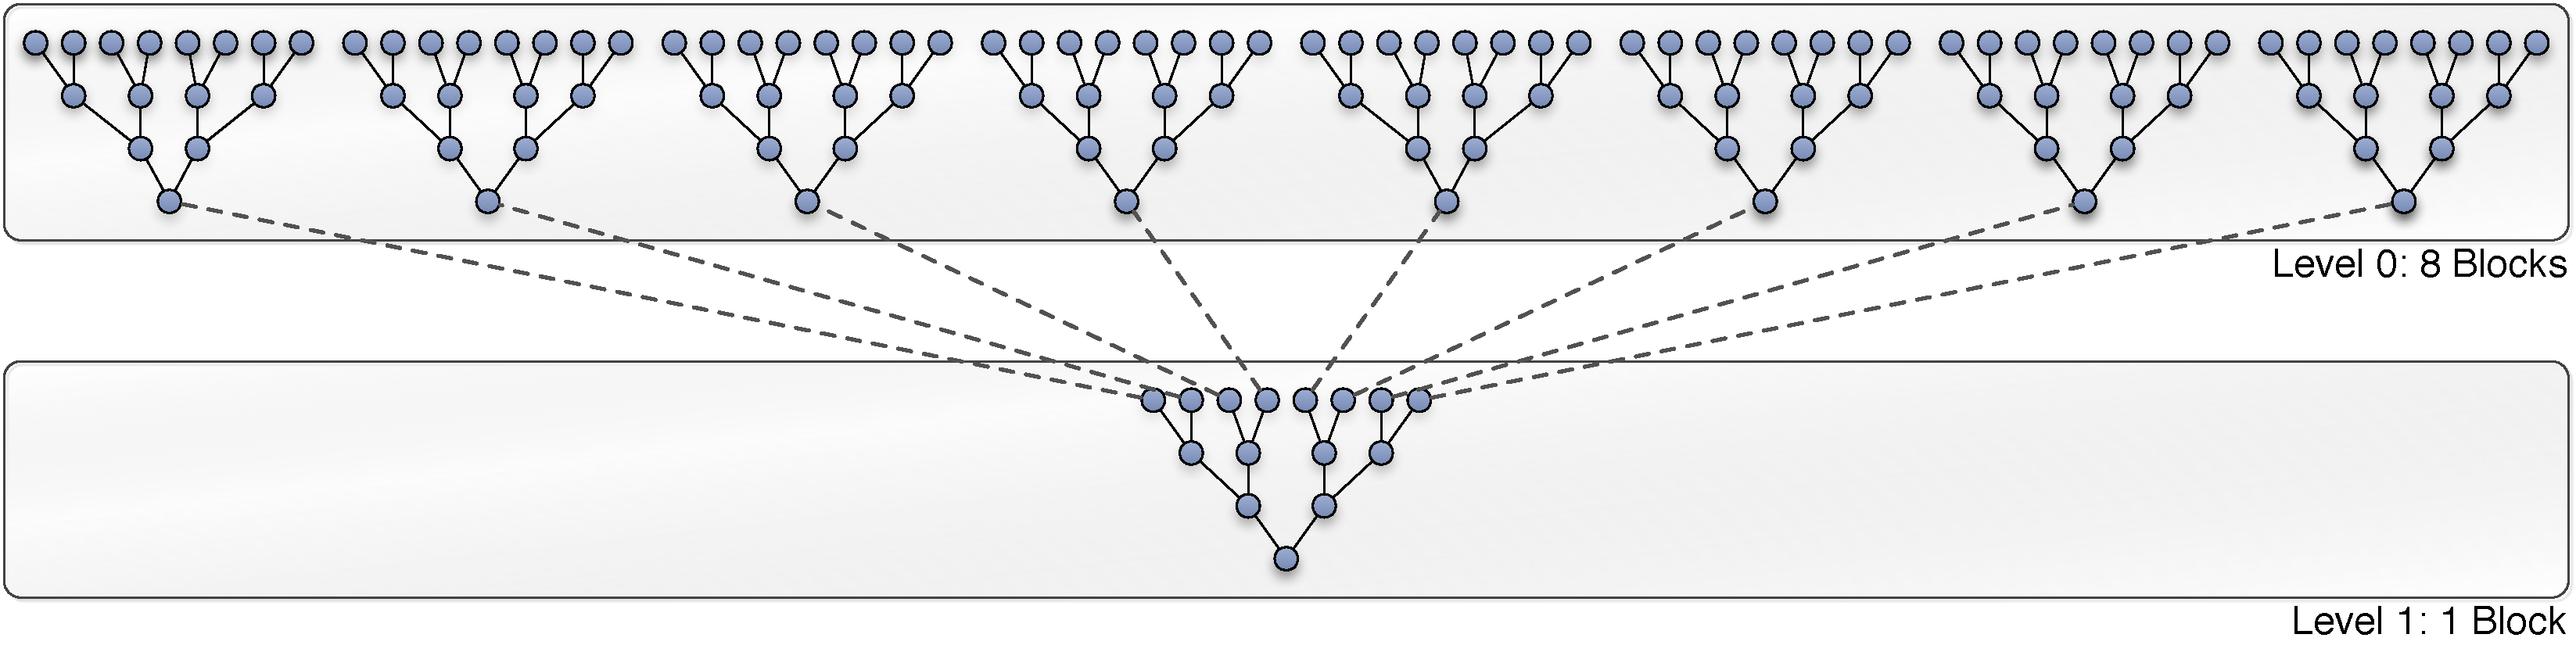
\includegraphics[width=\textwidth]{images/sec-4/tree-reduction}
    \end{center}
    \caption[A parallel tree reduction]{Illustration of a tree reduction,
        performed in two steps. In the first step 8 thread blocks in parallel
        reduce 8 elements to a single value. The thread blocks synchronise by
        writing their result to memory, and the kernel is called recursively
        until the final result is computed.}
    \label{fig:tree_reduction}
\end{figure}

For a fused dot product kernel, only the first line of reductions at level zero
perform the element wise multiplication. All subsequent reductions in that
kernel, as well as the recursive steps at level one and beyond, are pure
reductions. Thus, the fused operation requires compilation of two separate
kernels. % We focus on the level zero kernel, which is more interesting.

\subsubsection{Parallel Reduction Complexity}
\label{sec:parallel_reduction_complexity}

If each thread combines two elements at a time, then a vector of length $N$ will
be reduced in $\mathcal{O}\left( \log N \right)$ parallel steps. Each step $S$
does $\sfrac{N}{S^2}$ independent operations, so the \emph{step
complexity}\index{complexity!step} of the algorithm is:
\[
\mathcal{O}\left( \log N \right)
\]
For $N=2^{D}$, the algorithm thus performs $\sum_{S=1}^{D}2^{D-S} = N - 1$
operations. This means that the \emph{work complexity}\index{complexity!work} of
the algorithm is:
\[
\mathcal{O}\left( N \right)
\]
and so does not perform more work than a sequential algorithm. For $P$ threads
running physically in parallel on $P$ processors, the \emph{time
complexity}\index{complexity!time} is $\mathcal{O}\left( \sfrac{N}{P} + \log N
\right)$. In a thread block $N = P$, so the time complexity is:
\[
\mathcal{O}\left( \log N \right)
\]
Compare this to a sequential reduction, which has a time complexity of
$\mathcal{O}\left( N \right)$.

\subsubsection{Algorithm Cascading}
\label{sec:algorithm_cascading}

The \emph{cost} of a parallel algorithm is the number of processors $\times$
time complexity. This implies that the cost of the algorithm is
$\mathcal{O}\left( N \log N \right)$, which is \emph{not} cost efficient.

Brent's theorem~\cite{Chatterjee:2009vh} suggests that instead of each thread
summing two elements, \emph{algorithm cascading} can be used to combine a
sequential and parallel reduction. Each thread does $\mathcal{O}\left( \log N
\right)$ sequential work, which reduces the cost of the algorithm to
$\mathcal{O}\left( \sfrac{N}{\log N} \log N \right)$, or rather:
\[
\mathcal{O}\left( N \right)
\]
while keeping the work complexity $\mathcal{O}\left( N \right)$ and step
complexity $\mathcal{O}\left( \log N \right)$.

This suggests, for example, that a block of 256 threads should sum a total of
2048 elements. In practice it is beneficial to do even more sequential work per
thread, since this reduces the number of levels in the recursive tree reduction
and provides better latency hiding.



%\begin{itemize}
%    \item Accelerate frontend
%        \begin{itemize}
%            \item reification
%                \begin{itemize}
%                    \item smart constructors for type classes
%                    \item explicit dictionaries (polymorphism)
%                    \item environments
%                    \item HOAS vs. de Bruijn
%                    \item representation types
%                \end{itemize}
%            \item surface \& internal (core) languages
%                \begin{itemize}
%                    \item representing different constructs in surface/core
%                    \item surface nested $\rightarrow$ core flat ?? (fuuuuture)
%                \end{itemize}
%            \item sharing observation ( --> sec 5? not my work )
%        \end{itemize}
%
%    \item Accelerate CUDA backend
%        \begin{itemize}
%            \item code generation
%                \begin{itemize}
%                    \item architecture sensitive JIT cross-compiler
%                    \item future work: types, Haskell compile time
%                \end{itemize}
%            \item external compilation
%                \begin{itemize}
%                    \item annotating AST nodes
%                \end{itemize}
%            \item memory management
%                \begin{itemize}
%                    \item weak pointers \& weak hash tables
%                    \item advantages to alternatives
%                \end{itemize}
%            \item execution
%                \begin{itemize}
%                    \item occupancy analysis
%                    \item multi-pass kernels
%                \end{itemize}
%            \item performance
%                \begin{itemize}
%                    \item amortizing overheads (how to quantise this?)
%                    \item of generated code
%                    \item runtime overheads
%                    \item w.r.t. CUDA memory subsystem (theoretical performance)
%                    \item examples! spot the infelicities! (dot product)
%                \end{itemize}
%        \end{itemize}
%
%\end{itemize}
%
%Compilation has five phases:
%\begin{itemize}
%    \item Lexing
%    \item Parsing
%    \item Semantic analysis
%    \item Optimisation
%    \item Code Generation
%\end{itemize}

